\documentclass[a4paper]{article}

\usepackage[utf8]{inputenc}

\usepackage{multicol}
\usepackage{needspace}

\usepackage{tikz}
\usetikzlibrary{arrows,automata,trees,shapes,positioning,backgrounds,fit}
\tikzset{arrows={-triangle 45}}

\newcommand\eps{\ensuremath{\varepsilon}}

\newcommand{\regex}[1]{\texttt{#1}}

\newcommand{\pictable}[2]{%
\vspace{5pt}%
\begin{minipage}{0.47\linewidth}%
#1%
\end{minipage}%
\begin{minipage}{0.55\linewidth}%
#2%
\end{minipage}%
\vspace{5pt}%
}

\title{Converting Regular Expressions to\\ Discrete Finite Automata:\\ A Tutorial}
\author{David Christiansen}
\date{2013-01-03}

\begin{document}
\maketitle
This is a tutorial on how to convert regular expressions to nondeterministic
finite automata (NFA) and how to convert these to deterministic finite
automata. It's meant to be straightforward and easy to follow, rather than
worrying about every technical detail. Please see Torben Mogensen's book for
the nitty-gritty. In this tutorial, we write concrete regular expressions in
\regex{typewriter font} and variables ranging over regular expressions with
various forms of the letter $r$. The regular expression matching the empty
string is written \eps, pronounced ``epsilon''.  We use $\alpha$ and $\beta$,
pronounced ``alpha'' and ``beta'', to represent arbitrary symbols.


\section*{Converting Regular Expressions to NFAs}
\label{sec:conv-regul-expr}

A regular expression can consist of the following constructions:
\begin{itemize}
\item It can match the empty string, represented by \eps.
\item It can match a symbol $\alpha$ from the alphabet of the language to be matched.
\item It can match either of two regular expressions $r_1$ and $r_2$,
  written \regex{$r_1$|$r_2$}.
\item It can match a sequence of two regular expressions  $r_1$ and $r_2$,
  written \regex{$r_1$$r_2$}.
\item It can match zero or more instances of a regular expression
  $r$, written \regex{$r$*}.
\end{itemize}

We convert a regular expression to a nondeterministic finite automaton
(NFA) by considering each case in the above definition. By definition,
every automaton (whether NFA or DFA) has a \emph{single} start
state. An automaton may have more than one accepting state, but
because of the way the rules below are constructed, the resulting NFAs
will have exactly one accepting state.  Even if this were not the
case, it would be easy to create a unique accepting state by simply
creating a new unique accepting state and inserting \eps-transitions
from the previous accepting states to the new one.

\needspace{15cm} We begin with the base cases, that is, regular
expressions $\alpha$ and \eps.  The symbol $\alpha$ is matched by an
automaton that has a start state, an accepting state, and a transition
on $\alpha$ from the start state to the accepting state:

\begin{center}
  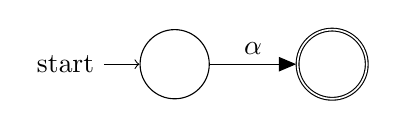
\begin{tikzpicture}[node distance=2cm, auto]
    \node[initial, state] (start) {};
    \node[accepting, state] (end) [right of=start] {};
    \path (start) edge node {$\alpha$} (end);
  \end{tikzpicture}
\end{center}

Because we are creating an NFA, we can use the same construction to
match the empty expression \eps, just with an \eps-transition to the
accepting state rather than a symbol from the alphabet. In other
words, the regular expression \eps\ gives rise to the following
automaton:

\begin{center}
  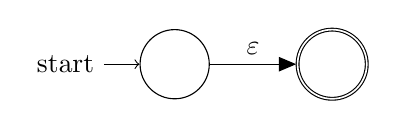
\begin{tikzpicture}[node distance=2cm, auto]
    \node[initial, state] (start) {};
    \node[accepting, state] (end) [right of=start] {};
    \path (start) edge node {$\eps$} (end);
  \end{tikzpicture}
\end{center}

In the remaining cases, that is, the composite regular expressions, we
need to represent the result of a recursive use of the conversion
procedure.  The result of converting some regular expression $r$ to an
NFA will be shown as follows:
\\
\begin{center}
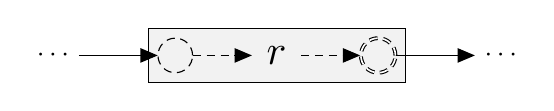
\begin{tikzpicture}[node distance=2cm, auto]
  \node (start) {$\cdots$};
  \begin{scope}[node distance=1cm, scale=0.5, transform shape, densely dashed]
    \node[state] (boxstart) [right = 2cm of start] {};
    \node (label) [right = 1.5 cm of boxstart, scale=3] {$r$};
    \node[state, accepting] (boxend) [right  = 1.5 cm of label] {};
    \path (boxstart) edge (label)
          (label) edge (boxend);
  \end{scope}
  \node (end) [right = 1cm of boxend] {$\cdots$};
  \path (start) edge (boxstart) (boxend) edge (end);
  \begin{pgfonlayer}{background}
    \node [
      fit=(boxstart) (boxend), fill=black!5, draw] {};
  \end{pgfonlayer}
\end{tikzpicture}
\end{center}
\noindent
The leftmost state in the box represents the start state of $r$'s automaton,
and the accepting state to the right represent the accepting states of $r$'s
automaton.

A choice between $r_1$ and $r_2$, written \regex{$r_1$|$r_2$}, is constructed
by creating a new start state with \eps-transitions to the start states of
$r_1$'s and $r_2$'s automata, and an accepting state with \eps-transitions from their
accepting states, as follows:
\begin{center}
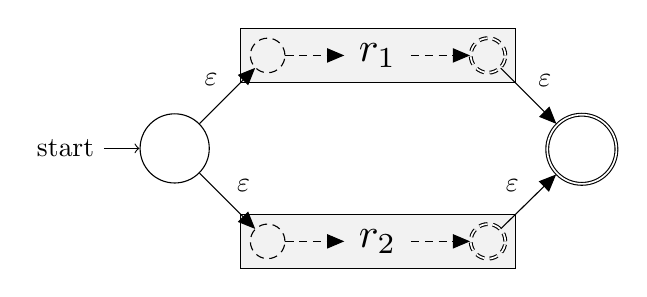
\begin{tikzpicture}[node distance=2cm, auto]

  \node [initial, state] (start) {};

  \begin{scope}[node distance=1cm, scale=0.5, transform shape, densely dashed]
    \node[state] (boxstart) [above right = 2cm of start] {};
    \node (label) [right = 1.5 cm of boxstart, scale=3] {$r_1$};
    \node[state, accepting] (boxend2) [right  = 1.5 cm of label] {};
    \path (boxstart) edge (label)
          (label) edge (boxend2);
  \end{scope}
  \begin{pgfonlayer}{background}
    \node [
%      shape=cloud, cloud puffs=10.8, cloud ignores aspect,
      fit=(boxstart) (boxend2), fill=black!5, draw] {};
  \end{pgfonlayer}
  \path (start) edge node {\eps} (boxstart);

  \begin{scope}[node distance=1cm, scale=0.5, transform shape, densely dashed]
    \node[state] (boxstart2) [below right = 2cm of start] {};
    \node (label2) [right = 1.5 cm of boxstart2, scale=3] {$r_2$};
    \node[state, accepting] (boxend22) [right  = 1.5 cm of label2] {};
    \path (boxstart2) edge (label2)
          (label2) edge (boxend22);
  \end{scope}
  \path (start) edge node {\eps} (boxstart2);
  \begin{pgfonlayer}{background}
    \node [
%      shape=cloud, cloud puffs=10.8, cloud ignores aspect,
      fit=(boxstart2) (boxend22), fill=black!5, draw] {};
  \end{pgfonlayer}

  \node[state, accepting] (end) [below right = 1 cm of boxend2] {};
  \path (boxend2) edge node {\eps} (end)
        (boxend22) edge node {\eps} (end);
\end{tikzpicture}
\end{center}

A sequence of two regular expressions $r_1$ and $r_2$, written $r_1r_2$, is
converted to an NFA by simply attaching the accepting states of $r_1$'s NFA to
the initial state of $r_2$'s NFA:

\begin{center}
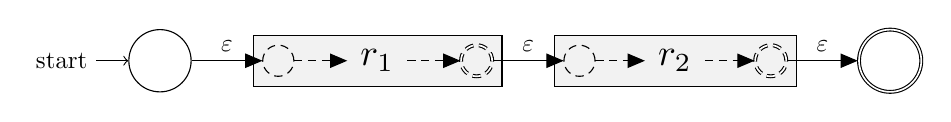
\begin{tikzpicture}[node distance=2cm, auto, scale=0.9, transform shape]

  \node [initial, state] (start) {};

  \begin{scope}[node distance=1cm, scale=0.5, transform shape, densely dashed]
    \node[state] (boxstart) [right = 2cm of start] {};
    \node (label) [right = 1.5 cm of boxstart, scale=3] {$r_1$};
    \node[state, accepting] (boxend2) [right  = 1.5 cm of label] {};
    \path (boxstart) edge (label)
          (label) edge (boxend2);
  \end{scope}
  \begin{pgfonlayer}{background}
    \node [
%      shape=cloud, cloud puffs=10.8, cloud ignores aspect,
      fit=(boxstart) (boxend2), fill=black!5, draw] {};
  \end{pgfonlayer}
  \path (start) edge node {\eps} (boxstart);

  \begin{scope}[node distance=1cm, scale=0.5, transform shape, densely dashed]
    \node[state] (boxstart2) [right = 2cm of boxend2] {};
    \node (label2) [right = 1.4 cm of boxstart2, scale=3] {$r_2$};
    \node[state, accepting] (boxend22) [right  = 1.4 cm of label2] {};
    \path (boxstart2) edge (label2)
          (label2) edge (boxend22);
  \end{scope}
  \begin{pgfonlayer}{background}
    \node [
%      shape=cloud, cloud puffs=10.8, cloud ignores aspect,
      fit=(boxstart2) (boxend22), fill=black!5, draw] {};
  \end{pgfonlayer}

  \node[state, accepting] (end) [right = 1 cm of boxend22] {};

  \path (boxend2) edge node {\eps} (boxstart2)
        (boxend22) edge node {\eps} (end);
\end{tikzpicture}
\end{center}

The NFA of the repeating expression \regex{$r$*} has an \eps-transition from
its start state to $r$'s start state, and an \eps-transition from $r$'s
accepting state to its accepting state. We allow unlimited repetitions of $r$
by inserting an \eps-transition from its accepting state to its start state,
and we allow $r$ to be skipped by inserting an \eps-transition from the new
start state directly to the new accepting state.

\needspace{10cm}
In picture form, the NFA corresponding to \regex{$r$*} is as follows:

\begin{center}
  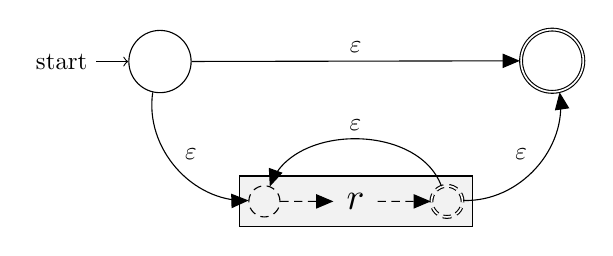
\begin{tikzpicture}[node distance=2cm, auto, scale=0.9, transform shape]
    \node[state, initial] (start) {};

    \begin{scope}[node distance=1cm, scale=0.5, transform shape, densely dashed]
      \node[state] (boxstart) [below right = 3cm and 2cm of start] {};
      \node (label) [right = 1.5 cm of boxstart, scale=3] {$r$};
      \node[state, accepting] (boxend) [right  = 1.5 cm of label] {};
      \path (boxstart) edge (label)
            (label) edge (boxend)
            ;
    \end{scope}
    \begin{pgfonlayer}{background}
      \node [fit=(boxstart) (boxend), fill=black!5, draw] {};
    \end{pgfonlayer}
    \path (boxend) edge [bend right=70] node [above] {\eps} (boxstart);
    \node[state, accepting] (end) [above right = 1.5cm and 1cm of boxend] {};
    \path (start) edge [bend right=50] node {\eps} (boxstart)
          (boxend) edge [bend right=50] node {\eps} (end)
          (start) edge  node {\eps} (end)
          ;
  \end{tikzpicture}
\end{center}


\section*{Converting NFAs to DFAs}

To convert an NFA to a DFA, we must find a way to remove all
\eps-transitions and to ensure that there is one transition per symbol
in each state. We do this by constructing a DFA in which \emph{each
  state corresponds to a set of some states} from the NFA\@.  In the
DFA, transitions from a state $S_1$ by some symbol $\alpha$ go to the
state $S_2$ that consists of all the possible NFA-states that could be
reached by $\alpha$ from some NFA state $q$ contained in the present
DFA state $S_1$.  The resulting DFA ``simulates'' the given NFA in the
sense that a single DFA-transition represents many simultaneous
NFA-transitions.

The first concept we need is the \eps-closure, pronounced ``epsilon
closure''.  The \eps-closure of an NFA state $q$ is the set containing
$q$ along with all states in the automaton that are reachable by any
number of \eps-transitions from $q$. In the following automaton, the
\eps-closures are given in the table to the right:

\pictable{
  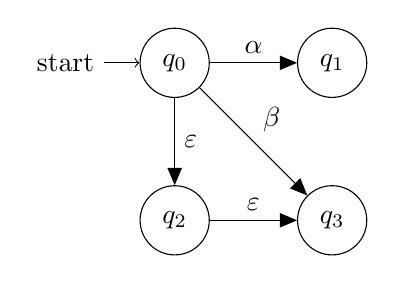
\begin{tikzpicture}[node distance=2cm, auto]
    \node[initial, state] (start) {$q_0$};
    \node[state] (two) [right of=start] {$q_1$};
    \node[state] (three) [below of =start] {$q_2$};
    \node[state] (four) [right of=three] {$q_3$};
    \path (start) edge node {$\alpha$} (two)
          (start) edge node {$\beta$} (four)
          (start) edge node {\eps} (three)
          (three) edge node {\eps} (four);
  \end{tikzpicture}
}{
\begin{tabular}{|c|l|}
  \hline
  State & \eps-closure\\
  \hline
  $q_0$ & $\{q_0, q_2, q_3\}$\\
  $q_1$ & $\{q_1\}$\\
  $q_2$ & $\{q_2, q_3\}$\\
  $q_3$ & $\{q_3\}$\\
  \hline
\end{tabular}
}
\noindent
Likewise, we can define the \eps-closure of a \emph{set of states} to
be the states reachable by \eps-transitions from its members. In other
words, this is the union of the \eps-closures of its elements.

To convert our NFA to its DFA counterpart, we begin by taking the \eps-closure
of the start state $q_0$ of our NFA and constructing a new
start state $S_0$ in our DFA corresponding to that \eps-closure.  Next, for each
symbol $\alpha$ in our alphabet, we record the set of NFA states that we can
reach from $S_0$ on that symbol.  For each such set, we make a DFA state
corresponding to its \eps-closure, taking care to do this only once
for each set.  In
the case two sets are equal, we simply reuse the existing DFA state that we already
constructed.  This process is then repeated for each of the new DFA
states (that is, set of NFA states)
until we
run out of DFA states to process.  Finally, every DFA state whose corresponding set
of NFA states contains an accepting state is itself marked as an accepting state.

\section*{Example}
\label{sec:example}

For this example, we'll convert the regular expression \regex{ba*b} into a
DFA. We being with simple automata matching \regex{a} and \regex{b}:

\begin{multicols}{2}
  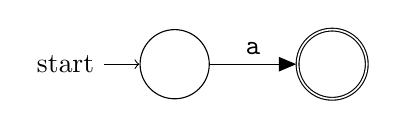
\begin{tikzpicture}[auto, node distance = 2cm]
    \node[initial, state] (a0) {};
    \node[accepting, state] (a1) [right of=a0] {};
    \path (a0) edge node {\regex{a}} (a1);
  \end{tikzpicture}

  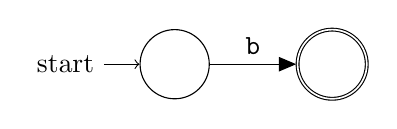
\begin{tikzpicture}[auto, node distance = 2cm]
    \node[initial, state] (a0) {};
    \node[accepting, state] (a1) [right of=a0] {};
    \path (a0) edge node {\regex{b}} (a1);
  \end{tikzpicture}
\end{multicols}

Next, we construct the automaton matching \regex{a*} using the automaton for
\regex{a}:

\begin{center}
  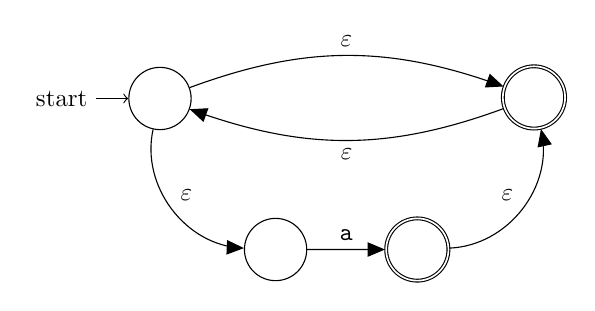
\begin{tikzpicture}[node distance=2cm, auto, scale=0.9, transform shape]
    \node[state, initial] (start) {};

      \node[state] (boxstart) [below right = 1.5cm and 1cm of start] {};
      \node[state, accepting] (boxend) [right of = boxstart] {};
      \path (boxstart) edge node {\regex{a}} (boxend);

    \node[state, accepting] (end) [above right = 1.5cm and 1cm of boxend] {};
    \path (start) edge [bend right=50] node {\eps} (boxstart)
          (boxend) edge [bend right=50] node {\eps} (end)
          (start) edge [bend left=20] node {\eps} (end)
          (end) edge [bend left=20] node {\eps} (start);
  \end{tikzpicture}
\end{center}

\needspace{10cm}
Finally, we attach our \regex{b}-automaton to each end using the rule for
sequencing:
\nopagebreak
\begin{center}
  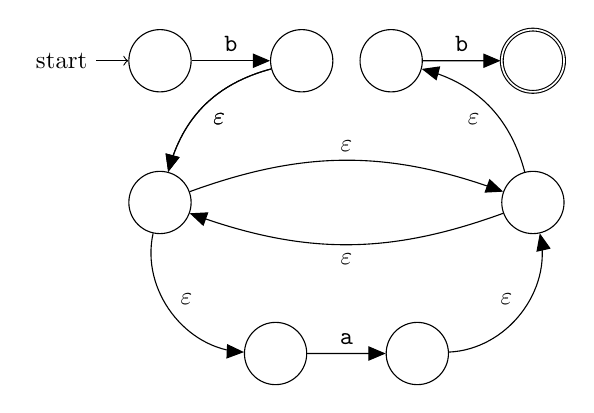
\begin{tikzpicture}[node distance=2cm, auto, scale=0.9, transform shape]
    \node[state, initial] (bstart) {};
    \node[state] (bend) [right of=bstart] {};
    \node[state] (starstart) [below of=bstart] {};
    \path (bstart) edge node {\regex{b}} (bend)
          (bend) edge [bend right] node {\eps} (starstart);

    \node[state] (boxstarstart) [below right = 1.5cm and 1cm of starstart] {};
    \node[state] (boxend) [right of = boxstarstart] {};
    \path (boxstarstart) edge node {\regex{a}} (boxend);

    \node[state] (end) [above right = 1.5cm and 1cm of boxend] {};
    \path (starstart) edge [bend right=50] node {\eps} (boxstarstart)
          (boxend) edge [bend right=50] node {\eps} (end)
          (starstart) edge [bend left=20] node {\eps} (end)
          (end) edge [bend left=20] node {\eps} (starstart);

    \node[state, accepting] (bend2) [above of=end] {};
    \node[state] (bstart2) [left of = bend2] {};
    \path (bstart2) edge node {\regex{b}} (bend2)
          (end) edge [bend right] node {\eps} (bstart2)
          (bend) edge [bend right] node {\eps} (starstart);
  \end{tikzpicture}
\end{center}

To convert this NFA to a DFA, we begin by labeling the states so we
can refer to them during the process:
\begin{center}
  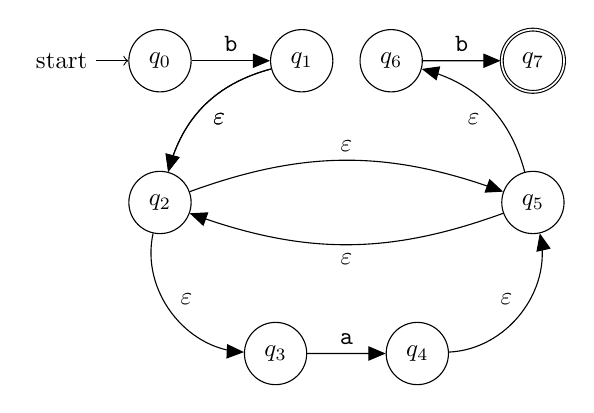
\begin{tikzpicture}[node distance=2cm, auto, scale=0.9, transform shape]
    \node[state, initial] (bstart) {$q_0$};
    \node[state] (bend) [right of=bstart] {$q_1$};
    \node[state] (starstart) [below of=bstart] {$q_2$};
    \path (bstart) edge node {\regex{b}} (bend)
          (bend) edge [bend right] node {\eps} (starstart);

    \node[state] (boxstarstart) [below right = 1.5cm and 1cm of starstart] {$q_3$};
    \node[state] (boxend) [right of = boxstarstart] {$q_4$};
    \path (boxstarstart) edge node {\regex{a}} (boxend);

    \node[state] (end) [above right = 1.5cm and 1cm of boxend] {$q_5$};
    \path (starstart) edge [bend right=50] node {\eps} (boxstarstart)
          (boxend) edge [bend right=50] node {\eps} (end)
          (starstart) edge [bend left=20] node {\eps} (end)
          (end) edge [bend left=20] node {\eps} (starstart);

    \node[state, accepting] (bend2) [above of=end] {$q_7$};
    \node[state] (bstart2) [left of = bend2] {$q_6$};
    \path (bstart2) edge node {\regex{b}} (bend2)
          (end) edge [bend right] node {\eps} (bstart2)
          (bend) edge [bend right] node {\eps} (starstart);
  \end{tikzpicture}
\end{center}

\needspace{5cm}\nopagebreak
We begin by taking the \eps-closure of the start state, $q_0$.  As
there are no epsilon transitions, we simply have the singleton set
$\{q_0\}$. Our DFA is as follows:

\pictable{
  \begin{center}
  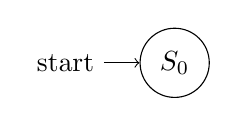
\begin{tikzpicture}
    \node[state, initial] (start) {$S_0$};
  \end{tikzpicture}
  \end{center}
}{
  \begin{tabular}{|c|c|c|l|}
    \hline
    State & \regex{a} & \regex{b} & NFA States\\
    \hline
    $S_0$ & ? & ? & $\{q_0\}$\\
    \hline
  \end{tabular}
}

The NFA state $q_0$ has no transitions on \regex{a}. Therefore, we mark this
table entry as an error. On a \regex{b}, it has a transition to $q_1$. The \eps-closure of
$q_1$ is $\{q_1, q_2, q_3, q_5, q_6\}$. We assign this set to a new DFA state
$S_1$, yielding the following automaton:

\pictable{
  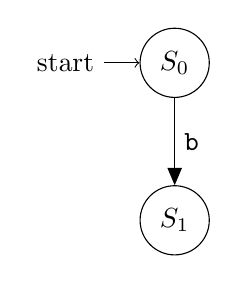
\begin{tikzpicture}[node distance = 2cm, auto]
    \node[state, initial] (q0) {$S_0$};
    \node[state] (q1) [below of = q0] {$S_1$};

    \path (q0) edge node {\regex{b}} (q1);
  \end{tikzpicture}
}{
  \begin{tabular}{|c|c|c|l|}
    \hline
    State & \regex{a} & \regex{b} & NFA States\\
    \hline
    $S_0$ & Err & $S_1$ & $\{q_0\}$\\
    $S_1$ & ? & ? & $\{q_1, q_2, q_3, q_5, q_6\}$\\
    \hline
  \end{tabular}
}

The NFA state $q_3$ has an \regex{a}-transition to $q_4$, which is the only
\regex{a}-transition in $S_1$'s NFA states. The \eps-closure of $q_4$
is $\{q_2, q_3, q_4, q_5, q_6\}$. The NFA state $q_6$ has the only
\regex{b}-transition in $S_1$'s NFA states, and it leads to $q_7$, whose
\eps-closure is simply $\{q_7\}$.

\pictable{
  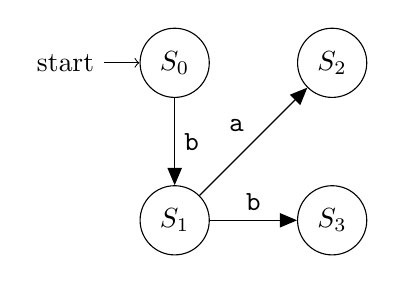
\begin{tikzpicture}[node distance = 2cm, auto]
    \node[state, initial] (S0) {$S_0$};
    \node[state] (S1) [below of = S0] {$S_1$};
    \node[state] (S2) [right of = S0] {$S_2$};
    \node[state] (S3) [right of = S1] {$S_3$};
    \path (S0) edge node {\regex{b}} (S1)
          (S1) edge node {\regex{a}} (S2)
          (S1) edge node {\regex{b}} (S3);
  \end{tikzpicture}
}{
  \begin{tabular}{|c|c|c|l|}
    \hline
    State & \regex{a} & \regex{b} & NFA States\\
    \hline
    $S_0$ & Err & $S_1$ & $\{q_0\}$\\
    $S_1$ & $S_2$ & $S_3$ & $\{q_1, q_2, q_3, q_5, q_6\}$\\
    $S_2$ & ? & ? & $\{q_2, q_3, q_4, q_5, q_6\}$\\
    $S_3$ & ? & ? & $\{q_7\}$\\
    \hline
  \end{tabular}
}

Analyzing $S_2$, we find an \regex{a}-transition from the NFA state $q_3$ to
the NFA state $q_4$.  However, we already have a DFA state corresponding to
$q_4$'s \eps-closure; namely, $S_2$ itself. Likewise, we have a
\regex{b}-transition to $q_7$, whose \eps-closure is represented by the DFA
state $S_3$.

\pictable{
  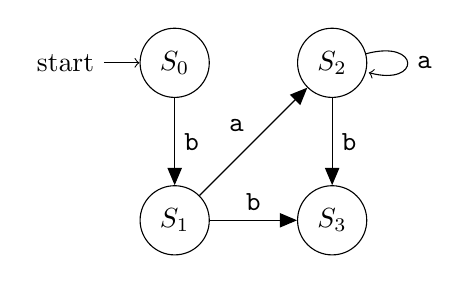
\begin{tikzpicture}[node distance = 2cm, auto]
    \node[state, initial] (S0) {$S_0$};
    \node[state] (S1) [below of = S0] {$S_1$};
    \node[state] (S2) [right of = S0] {$S_2$};
    \node[state] (S3) [right of = S1] {$S_3$};

    \path (S0) edge node {\regex{b}} (S1)
          (S1) edge node {\regex{a}} (S2)
          (S1) edge node {\regex{b}} (S3)
          (S2) edge [loop right] node {\regex{a}} (S2)
          (S2) edge node {\regex{b}} (S3);
  \end{tikzpicture}
}{
  \begin{tabular}{|c|c|c|l|}
    \hline
    State & \regex{a} & \regex{b} & NFA States\\
    \hline
    $S_0$ & Err & $S_1$ & $\{q_0\}$\\
    $S_1$ & $S_2$ & $S_3$ & $\{q_1, q_2, q_3, q_5, q_6\}$\\
    $S_2$ & $S_2$ & $S_3$ & $\{q_2, q_3, q_4, q_5, q_6\}$\\
    $S_3$ & ? & ? & $\{q_7\}$\\
    \hline
  \end{tabular}
}

Finally, we examine $S_3$, corresponding to $\{q_7\}$.  There are no outgoing
transitions from $q_7$, so we mark these as errors:

\pictable{
  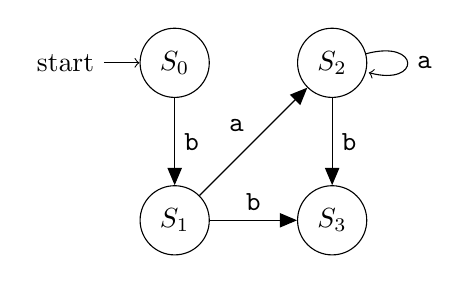
\begin{tikzpicture}[node distance = 2cm, auto]
    \node[state, initial] (S0) {$S_0$};
    \node[state] (S1) [below of = S0] {$S_1$};
    \node[state] (S2) [right of = S0] {$S_2$};
    \node[state] (S3) [right of = S1] {$S_3$};

    \path (S0) edge node {\regex{b}} (S1)
          (S1) edge node {\regex{a}} (S2)
          (S1) edge node {\regex{b}} (S3)
          (S2) edge [loop right] node {\regex{a}} (S2)
          (S2) edge node {\regex{b}} (S3);
  \end{tikzpicture}
}{
  \begin{tabular}{|c|c|c|l|}
    \hline
    State & \regex{a} & \regex{b} & NFA States\\
    \hline
    $S_0$ & Err & $S_1$ & $\{q_0\}$\\
    $S_1$ & $S_2$ & $S_3$ & $\{q_1, q_2, q_3, q_5, q_6\}$\\
    $S_2$ & $S_2$ & $S_3$ & $\{q_2, q_3, q_4, q_5, q_6\}$\\
    $S_3$ & Err & Err & $\{q_7\}$\\
    \hline
  \end{tabular}
}


Finally, we mark each DFA state (set of NFA states) as accepting if at
least one of its member NFA states are accepting.  In this case, only
$q_7$ is accepting, which means that only $S_3$ is accepting.

\pictable{
  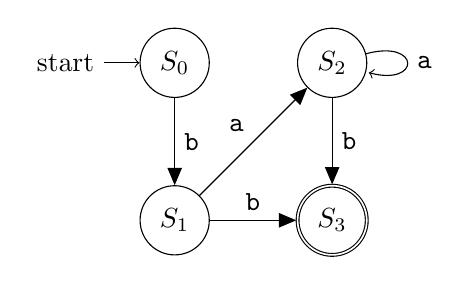
\begin{tikzpicture}[node distance = 2cm, auto]
    \node[state, initial] (S0) {$S_0$};
    \node[state] (S1) [below of = S0] {$S_1$};
    \node[state] (S2) [right of = S0] {$S_2$};
    \node[state, accepting] (S3) [right of = S1] {$S_3$};

    \path (S0) edge node {\regex{b}} (S1)
          (S1) edge node {\regex{a}} (S2)
          (S1) edge node {\regex{b}} (S3)
          (S2) edge [loop right] node {\regex{a}} (S2)
          (S2) edge node {\regex{b}} (S3);
  \end{tikzpicture}
}{
  \begin{tabular}{|c|c|c|l|}
    \hline
    State & \regex{a} & \regex{b} & Accepting\\
    \hline
    $S_0$ & Err & $S_1$ & No\\
    $S_1$ & $S_2$ & $S_3$ & No\\
    $S_2$ & $S_2$ & $S_3$ & No\\
    $S_3$ & Err & Err & Yes (from $q_7$)\\
    \hline
  \end{tabular}
}

The DFA is now fully constructed.

\section*{Acknowledgments}
\label{sec:acknowledgments}

I would like to thank Janus Varmarken for correcting an error in the first
version of this tutorial.
\end{document}



